\documentclass[conference]{IEEEtran}
\IEEEoverridecommandlockouts
% The preceding line is only needed to identify funding in the first footnote. If that is unneeded, please comment it out.
\usepackage{cite}
\usepackage{amsmath,amssymb,amsfonts}
\usepackage{float}
\usepackage{algorithmic}
\usepackage{graphicx}
\usepackage{enumitem}
\usepackage{textcomp}
\usepackage{xcolor}
\usepackage{hyperref}
\def\BibTeX{{\rm B\kern-.05em{\sc i\kern-.025em b}\kern-.08em
    T\kern-.1667em\lower.7ex\hbox{E}\kern-.125emX}}
    \pagestyle{plain}


\begin{document}

\title{Advanced Video Querying System for Machine Learning Applications}

\author{\IEEEauthorblockN{Vikas Kumar}
\IEEEauthorblockA{\textit{110156183} \\
\textit{University of Windsor}\\
Windsor, Canada \\
kumar3s@uwindsor.ca}
\and
\IEEEauthorblockN{Brendan Gignac}
\IEEEauthorblockA{\textit{110047251} \\
\textit{University of Windsor}\\
Windsor, Canada \\
gignac31@uwindsor.ca}
\and
\IEEEauthorblockN{Naman Bhagirathbhai Shah}
\IEEEauthorblockA{\textit{110156382} \\
\textit{University of Windsor}\\
Windsor, Canada \\
shah362@uwindsor.ca}
\and
\IEEEauthorblockN{Krish Jigarkumar Shah}
\IEEEauthorblockA{\textit{110156960} \\
\textit{University of Windsor}\\
Windsor, Canada \\
shah662@uwindsor.ca}
}

\maketitle

\begin{abstract}
The increasing volume of video data, exemplified by datasets like YouTube-8M\cite{abu2016youtube}, presents significant challenges for machine learning engineers, particularly in efficiently extracting relevant information for model training. Existing video querying systems often fall short in providing a comprehensive solution, lacking the ability to fetch relevant video sections and frames, analyze videos for effective searching, and store data in a centralized location. These limitations are particularly problematic for enterprises with large datasets, often composed of multiple sources, where new projects frequently emerge. Such projects require specific types of videos, such as those featuring cars or animals. Currently, meeting these changing needs necessitates reprocessing existing datasets or relying on previously assigned tags, which may not capture the full range of complex interactions. In response to these challenges, we propose a video querying system that enables precise searches within large-scale video datasets. Our solution employs Yolo11~\cite{yolo11} for object detection and tracking, generating detailed metadata that includes bounding box coordinates and timestamps. This metadata is stored in a MongoDB\cite{mongodb} database, allowing users to perform complex queries, such as identifying when a person and a car are within 10 pixels of each other. By optimizing the retrieval of relevant video segments and enhancing the tagging process, our system aims to meet the evolving needs of enterprises while leveraging the current technological capabilities of the Yolo11~\cite{yolo11} model.
\end{abstract}

\begin{IEEEkeywords}
Video Querying, Machine Learning, Object Detection, Temporal and Spatial Searches, Big Data, stream, frames
\end{IEEEkeywords}

% Introduction (5% points)
% Statement of the project purpose must be clearly and completely described. Summarize
% everything done in phase 1 (except Abstract) under this heading (with sub-headings).
% You may need to restructure and redraft this section. Make sure that aim, objectives
% and uniqueness of your work is clearly given.

\section{Introduction}

\subsection{Purpose of the Project}

With the increasing volume of video data, massive datasets like YouTube-8M\cite{abu2016youtube} present significant challenges for machine learning engineers due to their size and complexity. Processing entire datasets for training AI models is highly resource-intensive and often impractical. There is a need for an advanced system that can effectively filter and retrieve only the most relevant video segments for targeted machine-learning purposes.

\subsection{Problem Statement}

Current video querying solutions offer basic features like object detection and simple temporal tagging but lack sophisticated capabilities such as spatial querying and detecting interactions between multiple objects. They are unable to handle complex queries such as identifying when a person and a car are within a specific proximity or when two objects appear in a scene together within a specific time frame. This project addresses these limitations by creating an efficient system that filters massive datasets and extracts specific segments needed for AI model training.

\subsection{Motivation}

The growing complexity of video data requires precise and efficient querying tools to facilitate AI model training. Such tools are essential in domains like autonomous driving, surveillance, and content recommendation. By enabling precise data extraction, our system aims to reduce computational resources and accelerate AI development cycles, leading to more efficient and accurate machine learning processes.

\subsection{Aim}

The aim of this project is to develop a comprehensive video querying system capable of performing precise spatial-temporal queries and detecting complex object interactions. This system is designed to serve as a targeted data filtering mechanism, enhancing the efficiency of AI training workflows and reducing resource consumption.

\subsection{Objectives}

The primary objectives of the project are:

\begin{itemize}
    \item Enable Precise Temporal and Spatial Queries: Allow users to search for moments in videos based on time intervals and spatial locations.
    \item Support Complex Object Interaction Queries: Facilitate searches involving multiple objects and their interactions.
    \item Provide Efficient Data Filtering for Machine Learning: Serve as a system to filter data segments needed for training, conserving resources and optimizing workflows.
\end{itemize}
   
\subsection{Approach}

The system integrates state-of-the-art object detection and tracking technologies into a queryable video database application. It involves:

\begin{itemize}
    \item Video Ingestion: Videos are uploaded and processed using Yolo11\cite{yolo11} to detect objects.
    \item Metadata Generation: Detailed metadata, including spatial and temporal tags, is stored in MongoDB\cite{mongodb}.
    \item Query Engine: Supports temporal and spatial searches based on the stored metadata.
    \item Feature Engineering: Detailed metadata, bounding box coordinates, and timestamps are generated, with spatial indexing (using R-trees) and temporal indexing implemented to enable efficient querying.
\end{itemize}

\subsection{Experimental Setup and Demonstration}

The system will be tested using diverse video datasets to demonstrate its ability to handle large-scale data, and perform efficient queries.

\subsection{System Workflow}

The video management system involves:

\begin{itemize}
    \item Video Upload and Storage: Video is divided into smaller chunks and stored in MongoDB GridFS\cite{mongodb_gridfs}, with metadata saved in MongoDB\cite{mongodb}.
    \item Metadata and Querying: Users can query the video data through a query processor that responds with relevant metadata and video access links.
    \item Video Retrieval: The user can fetch specific video chunks based on the query.
\end{itemize}

By providing a system that performs complex temporal and spatial queries and efficiently retrieves video data, this project addresses a critical open sourced need in managing large-scale datasets for machine learning making it a valuable tool for engineers and researchers alike.

\section{Literature Review}
Currently, there is no open-source framework that efficiently retrieves relevant video segments based on content analysis. Existing closed solutions primarily focus on video analysis, returning metadata that users must store and process independently. This necessitates the creation of a pipeline to segment videos into required portions and convert them into frames, leading to a repetitive and resource-intensive process. Without such pipelines, significant computational resources may be wasted processing irrelevant content, often forcing users to restart the analysis from scratch for each new use case.\\
\par 
The closest tool addressing this issue is Scanner\cite{poms2018scanner}, which provides flexibility and allows the integration of various machine-learning models. Scanner\cite{poms2018scanner} efficiently processes large video datasets, making it suitable for applications such as 3D pose estimation, VR video synthesis, and large-scale video data mining. However, it still requires reprocessing the entire video when use cases change, despite having techniques to minimize irrelevant frames.\\
\par 
Major platforms like Google and IBM offer video analysis services but lack integrated storage, querying, and streaming solutions. Clients must upload videos to these platforms and expend resources developing their own solutions for these tasks.\\
\par 
In the realm of video database management systems (VDBMS), several legacy systems exist that allow content-based querying of video frames. However, many of these platforms have become obsolete due to advancements in video analysis techniques and codecs that offer superior compression. Consequently, they have failed to adapt to evolving technological standards.
\\\par
\begin{table*}[t] % Use table* for spanning both columns
    \centering
    \caption{This table shows the different features provided by the existing projects that are relevant to our problem space.}
    \label{tab:training_results}
    \resizebox{\textwidth}{!}{% Automatically resize to fit the full page width
    \begin{tabular}{lcccccccc}
        \hline
        \textbf{} & \textbf{TransVOD} & \textbf{TansVod++} & \textbf{TransMOT} & \textbf{BilVideo} & \textbf{VIMS} & \textbf{VDBMS} & \textbf{Online Platforms- Video Analysis} & \textbf{Our Solution} \\
        \hline
        Analysis &Y & Y &Y & N(Manual) & (TAg Based) & Y & Y &Y\\
        Storage & N & N &N & Y & Y & Y & N &Y\\
        Metadata Query & Y & Y &Y & Y & Y & Y & N&Y\\
        Metadata storage & N& N &N & Y & Y & Y & N &Y\\
        Streaming& N& N &N & Y & Y & Y & N &Y\\
        Chunk Streaming  & N &N & N & N & N & N& N &Y\\
        \hline
    \end{tabular}%
    }
\end{table*}
\begin{itemize} [itemsep=5pt]
    \item VDBMS\cite{aref2003vdbms}: This platform introduces video as a fundamental data type, supporting image similarity search and video streaming, but it primarily focuses on storage and does not serve data in formats conducive to machine learning, returning the entire video instead.
    \item BilVideo\cite{ozsoyoglu2003bilvideo}: Their analysis process, termed "fact-extraction," is semi-automatic, requiring users to manually specify objects in video frames using minimum bounding rectangles (MBRs). However, as an older platform, it lacks modern analysis capabilities.
    \begin{figure}[h!]
        \centering
        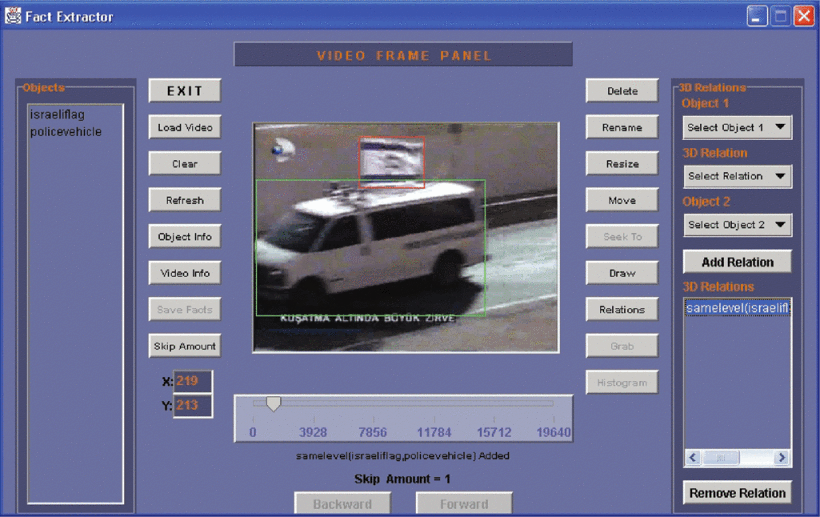
\includegraphics[width=0.5\textwidth]{BilVideo.png}
        \caption{Screenshot Demonstration of BilVideo System}
        \label{fig:bilvideo_demo}
    \end{figure}
    \item VIMS\cite{lee1997vims} This system employs a completely manual process for analysis and object detection, making it less efficient.
    \item YOLO11 \cite{yolo11} leverages transformer-based attention mechanisms to enhance spatial-temporal feature extraction, boosting accuracy in complex video analysis. Its anchor-free design improves object localization, while neural architecture search (NAS) fine-tunes the model’s structure for optimal performance. Multi-scale and multi-query processing further elevate detection across diverse scenes, ensuring robustness in varying contexts.
    \item TransVOD\cite{zhou2022transvod} utilizes spatial-temporal transformers for object detection and tracking, emphasizing relevant feature extraction through attention mechanisms.
    \item TransVOD++\cite{zhou2023transvodplusplus} enhances feature fusion, improving spatial and temporal integration for better contextual understanding. Its refined attention mechanisms dynamically focus on critical features, while multi-scale processing enhances detection of varying object sizes. Advanced training methodologies further improve generalization.
    \item TransMOT\cite{chu2021transmot} specializes in multi-object tracking using graph transformers, effectively capturing spatial relationships but lacking comprehensive querying capabilities.
    \item BoostTrack\cite{stanojevic2024boostTrack} emphasizes real-time tracking using efficient algorithms like DeepSORT, excelling in accuracy but limited in broader detection tasks.
    \item AQATrack\cite{xie2024autoregressivequeriesadaptivetracking} focuses on single-object tracking, achieving high accuracy but struggling with interactions among multiple objects.\\
\end{itemize}
\par
The individual differences compared to our solution have been shown in Table~\ref{tab:training_results}.
\par
YOLO11 leverages neural architecture search (NAS) and transformer-based models to enhance object detection accuracy in video queries. By integrating attention mechanisms, YOLOv11 ensures precise localization and efficient real-time video analysis. Its flexible, anchor-free detection system, combined with transformers for improved query handling, sets a new benchmark for performance in dynamic video and image analysis tasks\cite{yolo11}.

\section{Our Solution}
\subsection{Explanation of the Model}

The project aimed to develop a comprehensive video querying system designed to enable precise spatial-temporal queries and support complex multi-object interactions in large-scale video datasets. The core idea of this system is to extract and index relevant metadata for each video frame, including object locations, timestamps, and interactions, making it possible to search for specific events based on user-defined criteria.



\subsection{Workflow Overview}

The system’s workflow consists of the following key stages
\begin{itemize} [itemsep=5pt]
    \item Video Ingestion: Users upload videos to the system through APIs. Videos are pre-processed and segmented for transfer efficiency and relevant segment retrieval.
    \item Object Detection and Metadata Generation: Using YOLO11\cite{yolo11}, the system detects objects in each frame, identifies their spatial coordinates (bounding boxes), and timestamps their occurrences. Then we process this data to track the object over the video using our Algorithm described in the next section.
    \item Metadata Storage: The generated metadata, including spatial-temporal data and object identifiers, is stored in MongoDB\cite{mongodb}.
    \item Query Processing: Users can input spatial-temporal queries through a query engine. This engine processes the queries by searching the stored metadata and retrieving relevant video segments based on user-defined conditions.
    \item Result Presentation: The system provides access to the retrieved video segments or specific frames that match the query criteria.
\end{itemize}


\begin{figure}[h!]
    \centering
    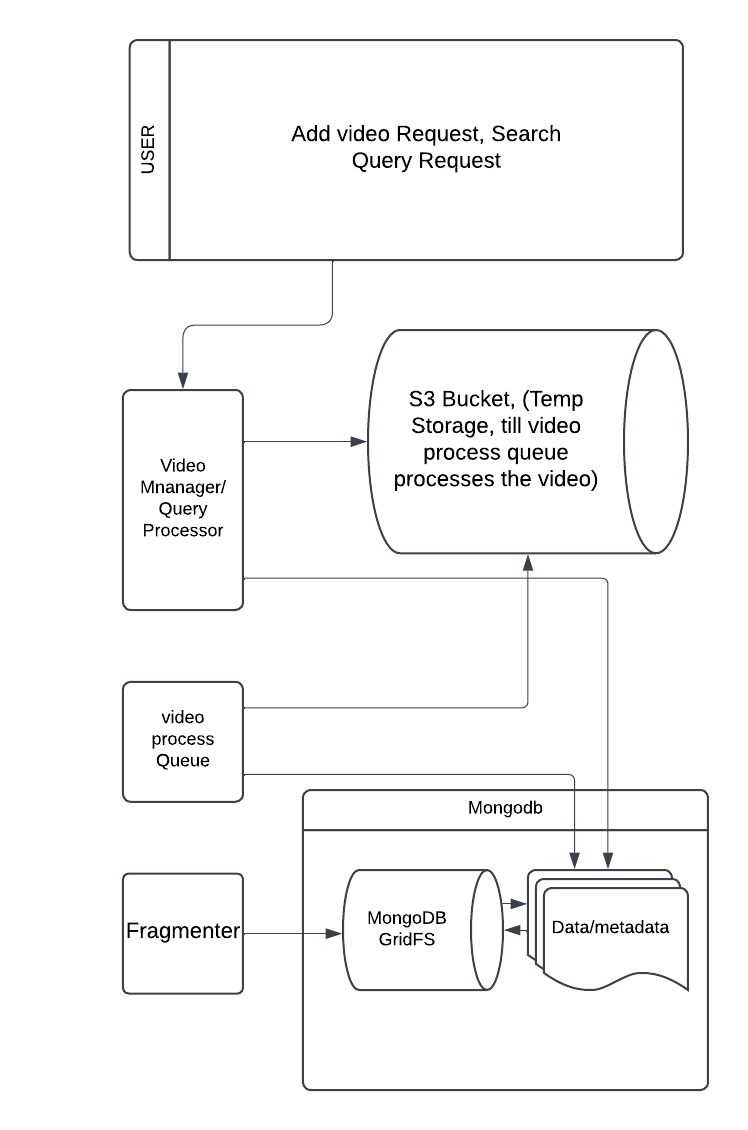
\includegraphics[width=0.5\textwidth]{architecture.png}
    \caption{Architecture Diagram}
    \label{fig:data_flow}
\end{figure}

\subsection{Workflow Explanation}

The workflow diagram illustrates the architecture and operation of the Video Management System.
\begin{figure}[h!]
\centering
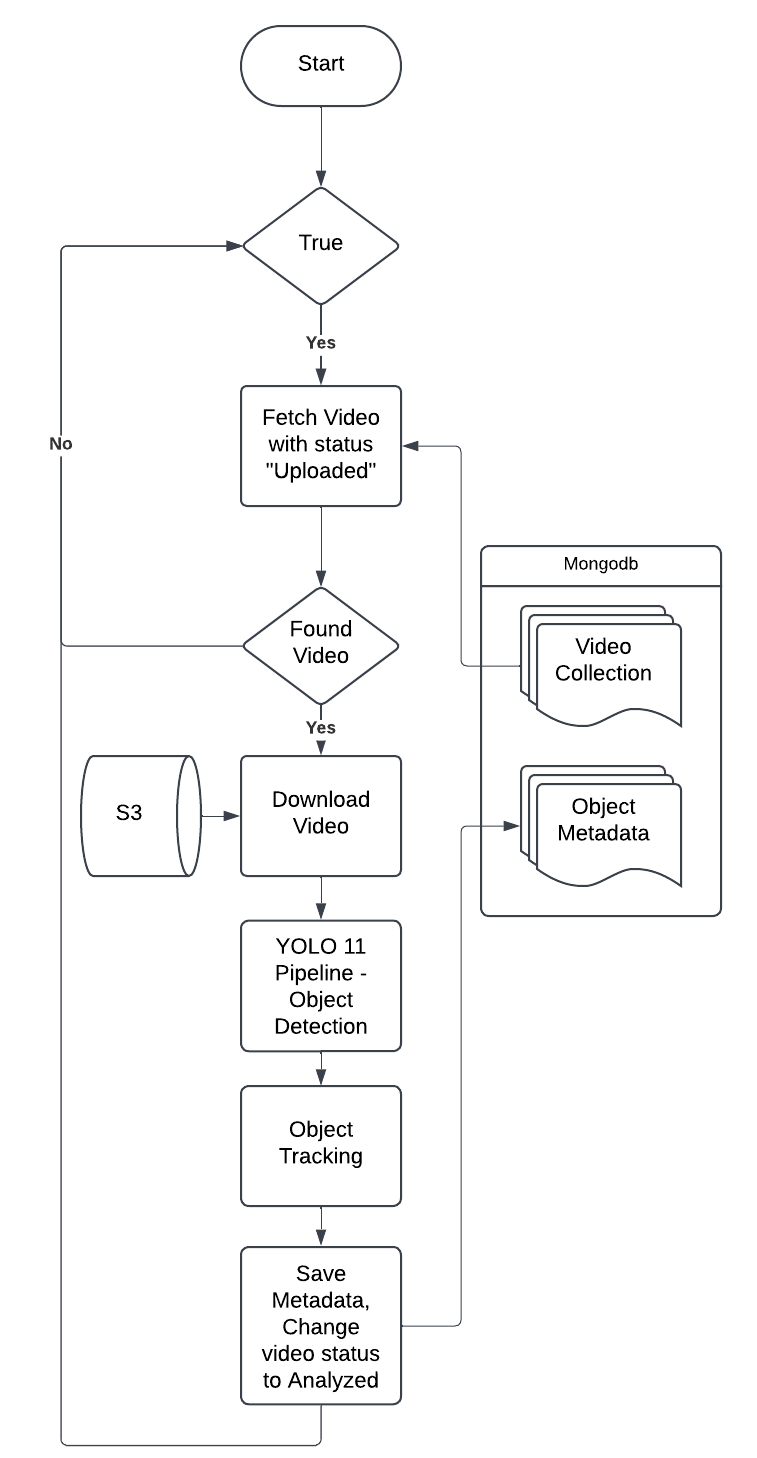
\includegraphics[width=0.5\textwidth]{analyze.png}
\caption{Analysis Pipeline Program Flowchart}
\label{fig:analyze_flow}
\end{figure}
\begin{itemize}[itemsep=5pt]
    \item User Requests to Upload a Video: The user initiates the process by requesting to upload a video. The user provides a title description of the video.
    \item Save Video Details in MongoDB\cite{mongodb}: The program saves the user-provided data (such as video title, upload date, etc.) in the MongoDB\cite{mongodb} database in collection videos. The server responds to the user with the generated ID.
    \item Upload: The user uploads the video at the upload link and provides the video ID.
    \item S3: Once the video is uploaded it is sent to s3 so that other services like Analyzer and then Fragmenter can access it.
    
    \item Analyzer: It processes the video to extract meaningful metadata using YOLO11. The metadata extracted only contains information about object locations and relative positions. We created our algorithm that uses Intersection over union as the backbone to track objects over time.
    \item More processing Pipelines can be added here Along with an Analyzer that specializes in different categories based on the needs and processing power available.
    \item Fragmenter: It divided the video into smaller 5-second chunks and stored efficiently in MongoDB GridFS\cite{mongodb_gridfs}. GridFS further breaks these fragments into 5 MB chunks which minimizes the loss.
\end{itemize}

Now video is available to query. We created 5 types of queries that can solve many kinds of problems related to searching in video.
\begin{itemize}[itemsep=5pt]
    \item User Queries through APIs: We provide REST APIs that the user has to use in order to get the relevant timestamps of the video.
    \item The queries utilize objects collection of MongoDB which contains the metadata. This metadata is processed on both MongoDB and query processor which is written in Nodejs.
    \item Download video: The user can use this timestamp value to download the videos, only the relevant section of the video will be returned to the user.
\end{itemize}
\begin{figure}[h!]
\centering
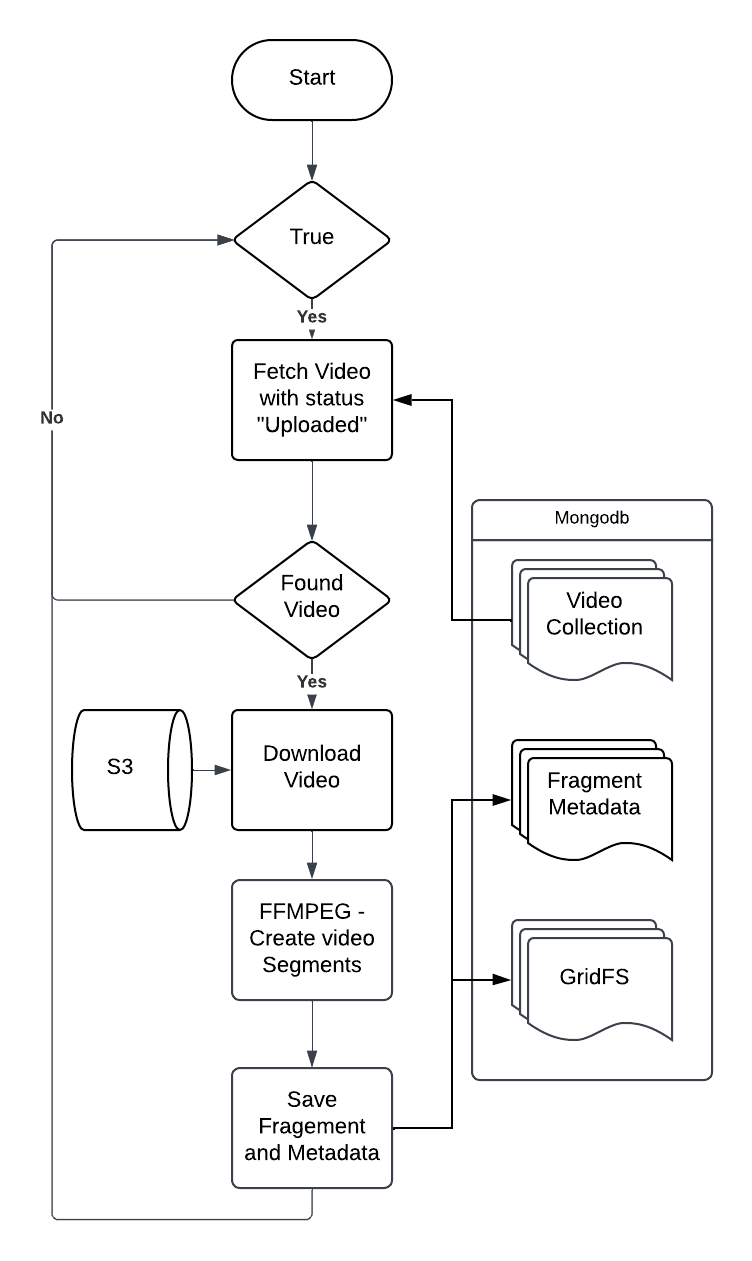
\includegraphics[width=0.5\textwidth]{Fragmenter.png}
\caption{Fragmenter Pipeline Program Flowchart}
\label{fig:upload_flow}
\end{figure}
The diagram emphasizes the integration of video storage, efficient metadata management, and a robust querying process to achieve precise and fast video retrieval based on user-defined spatial and temporal conditions. This architecture ensures that large videos are managed efficiently, enabling seamless upload, storage, and querying operations

\subsection{Differences from Existing Works}

Existing commercial video querying services, notably Google Cloud Video Intelligence API\cite{google_video_intelligence} and IBM Watson Video Enrichment\cite{ibm_watson_video_enrichment}, primarily focus on basic general object detection and simple tagging but do not offer advanced querying capabilities. They do not support user-defined complex queries involving multi-object interactions, precise spatial proximity, or movement tracking across regions and time intervals among more specialized complex use cases.

Our model differs by providing:

\begin{itemize}
    \item Customizable Spatial-Temporal Queries: Users can search for moments based on both spatial regions within video frames and specific time intervals.
    \item Multi-Object Interaction Detection: The system allows users to define and search for interactions between multiple objects.
    \item  Context-Aware Spatial Region Queries: Enables context-aware searches based on specific regions and actions within those regions.
    \item Efficient Data Filtering for ML Applications: It filters and extracts only the required video segments, reducing the computational load for targeted AI training.
\end{itemize}

\subsection{Features of the Product}

\begin{itemize}
    \item Precise Spatial and Temporal Querying: The system can identify objects based on user-defined spatial coordinates within a video frame and specific timestamps. Example: "Find moments when a car enters the top-left quadrant between 2 and 3 minutes."
    \item Multi-Object Interaction Detection: Enables searches for specific interactions between objects, such as "Find all moments when a person and a bicycle are within 10 pixels of each other."
    \item Context-Based Spatial Region Queries: Supports querying based on objects' movements and actions within specific regions of the frame. Example: "Identify moments when a person enters the bottom-right quadrant and remains there for 5 seconds."
    \item Efficient Indexing and Metadata Storage: Uses a combination of spatial (R-trees) and temporal (B-tree) indexing for efficient data storage and retrieval.
\end{itemize}


\subsection{Important Feature: Metadata Table for Complex Spatial-Temporal Queries}

The metadata table serves as a crucial feature of the video querying system, as it efficiently organizes and indexes information about events detected within the videos. Each row in the table represents a specific event, object, or action that occurs in a video, along with key details necessary for precise spatial-temporal querying.

\section{Metadata Schema}
\begin{figure}[H]
    \centering
    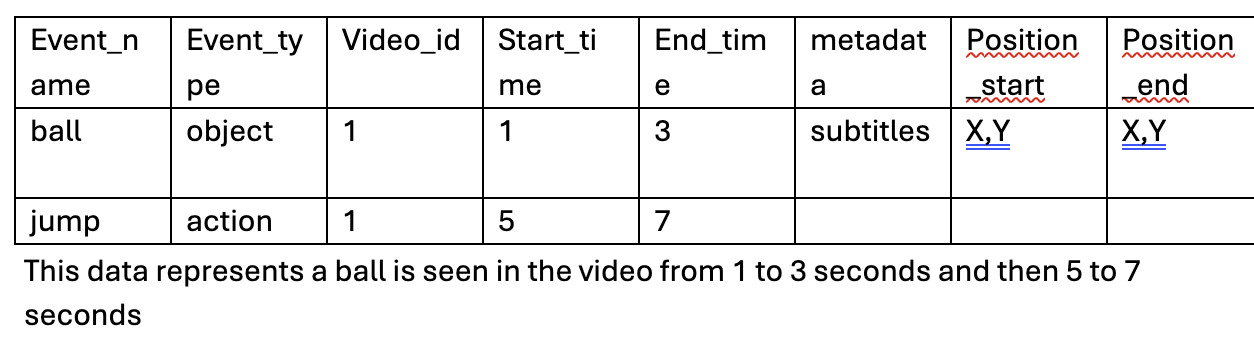
\includegraphics[width=0.5\textwidth]{metadata_schema.png} 
    \caption{Metadata Schema for Video Querying System}
    \label{fig:metadata-schema}
\end{figure}

Here’s an explanation of the table’s components:
\begin{itemize}[itemsep=5pt]
    \item Event Name: Identifies the type of event or object (e.g., "ball" or "jump").
    \item Event Type: Specifies whether the entry is an "object" (stationary or moving) or an "action" (a specific event like jumping).
    \item Video ID: A unique identifier for the video where the event occurs, allowing for cross-referencing between different videos in the database.
    \item Start Time and End Time: These columns denote the time interval in the video where the event is observed. For example, the "ball" appears between seconds 1 and 3 in the video, and the "jump" action is observed between seconds 5 and 7.
    \item Metadata: Provides additional context about the event, such as "subtitles," which could include descriptions or dialogue related to the event.
    \item Position Start and End: Records the spatial coordinates of the event at the start and end times. This information is essential for tracking movements or interactions within the frame. For instance, the coordinates (X, Y) help the system determine where in the frame the "ball" appears and whether it moves or remains stationaryc.
\end{itemize}
    
In the example Metadata Schema table, we see two events:
    A ball is seen from 1 to 3 seconds in the video, located at specific coordinates within the frame.
    A jump action occurs from 5 to 7 seconds, representing an action that can be queried based on time.
The metadata table enables the system to perform complex queries such as:
    "Find all instances where a ball is within a specific region of the frame between seconds 1 and 3."
The screenshot of the table effectively showcases the organized structure of the event metadata. By linking spatial-temporal data with detailed object and action information, this feature allows the system to efficiently handle and retrieve specific video segments based on user-defined conditions. This approach significantly enhances the accuracy and flexibility of the video querying process.


\section{Results}
\label{sec:results}
Our system implements several query endpoints that enable precise video content retrieval.

Users can specify where the object should be present in the video by using the predefined positions: "top-half", "bottom-half", "left-half", "right-half", "top-third", "middle-third-horizontal", "bottom-third", "left-third", "middle-third-vertical", "right-third", "top-left", "top-right", "bottom-left" and "bottom-right".

\subsection{Download Segment Query}
\textbf{Endpoint:} \\
\texttt{/query/chunk/download/:chunk\_id}

This endpoint provides support to other search queries by allowing the user to download the specific chunk based on its ID. The ID of the chunk is returned by the search APIs. Once the user has these IDs they can choose to download the chunk which is playable as a video. By requesting multiple chunks from the same video the user can create the whole video.

\subsection{Spatial Object Queries}
\textbf{Endpoint:} \\ 
\texttt{/query/spatialObjects}

This endpoint enables querying for objects within specified spatial regions. It implements a logical OR operation to find instances of any specified objects in the defined area.

\textbf{Parameters:}
\begin{itemize}
    \item \texttt{objects}: Array of object names (e.g., ["truck", "handbag"])
    \item \texttt{area}: Predefined area (e.g., "left-half") or coordinate array
\end{itemize}

Example queries:\\
\begin{minipage}{\linewidth}
\scriptsize
\begin{verbatim}
/query/spatialObjects?objects=["truck","handbag"]
&area=left-half
\end{verbatim}
\end{minipage}

\begin{figure}[H]
    \centering
    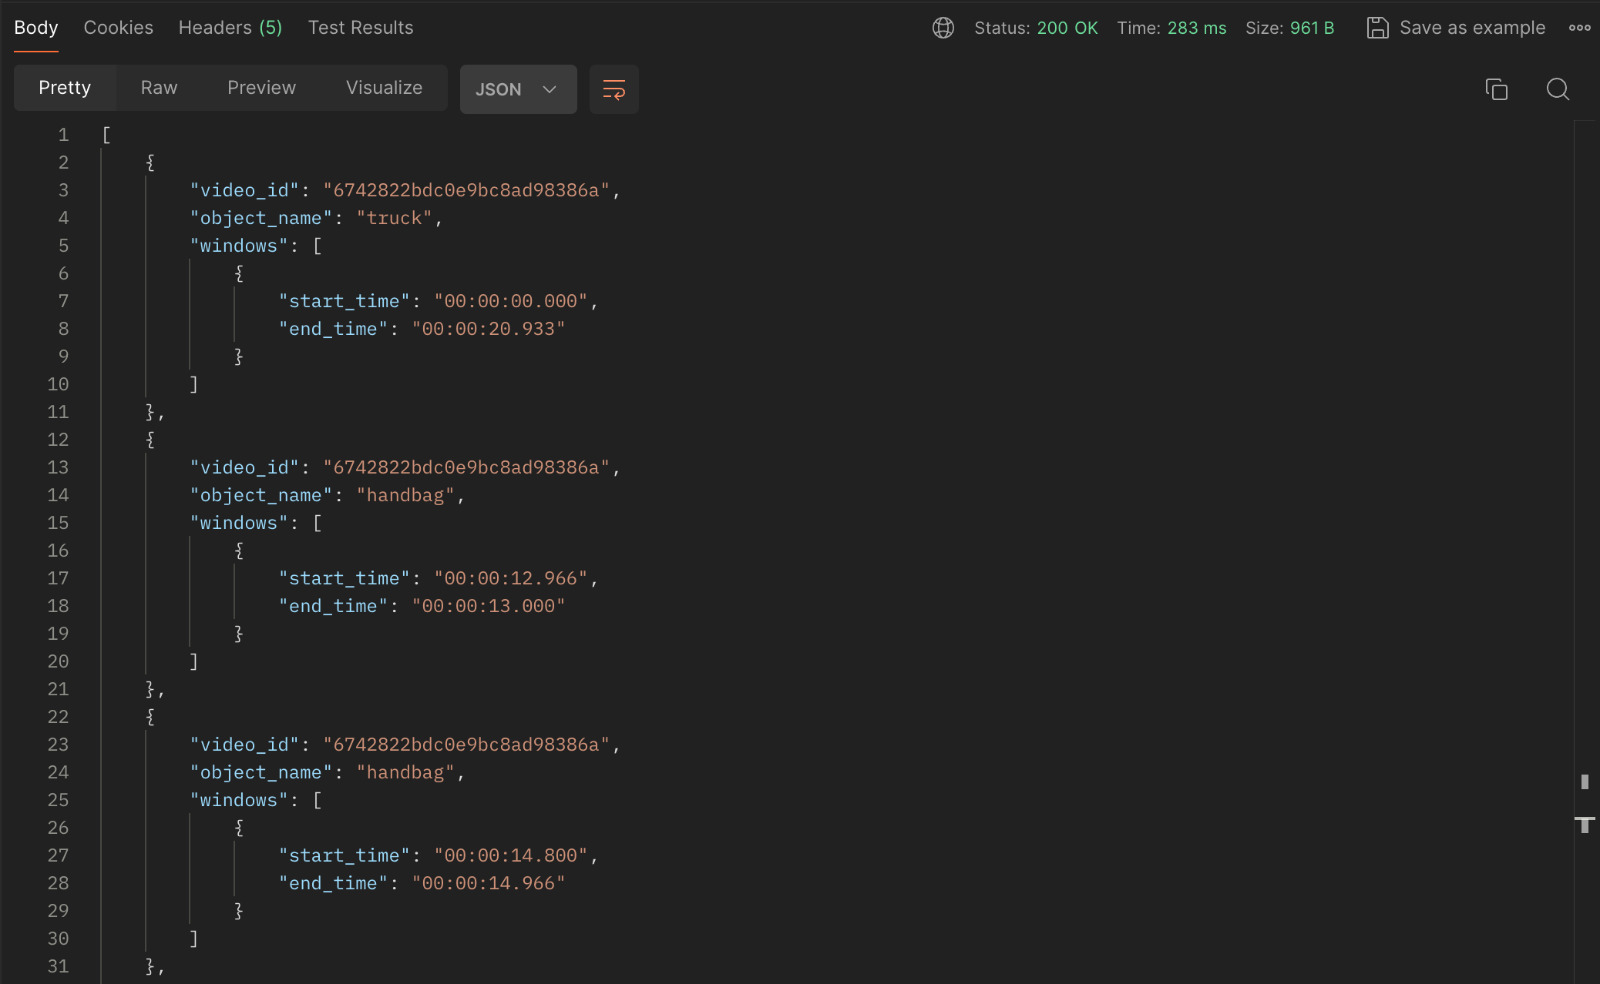
\includegraphics[width=0.45\textwidth]{1.jpeg}
    \caption{Result of spatial query for truck and handbag in left half}
    \label{fig:query1}
\end{figure}

\begin{minipage}{\linewidth}
\scriptsize
\begin{verbatim}
/query/spatialObjects?objects=["person"]
&area=bottom-right
\end{verbatim}
\end{minipage}

\begin{figure}[H]
    \centering
    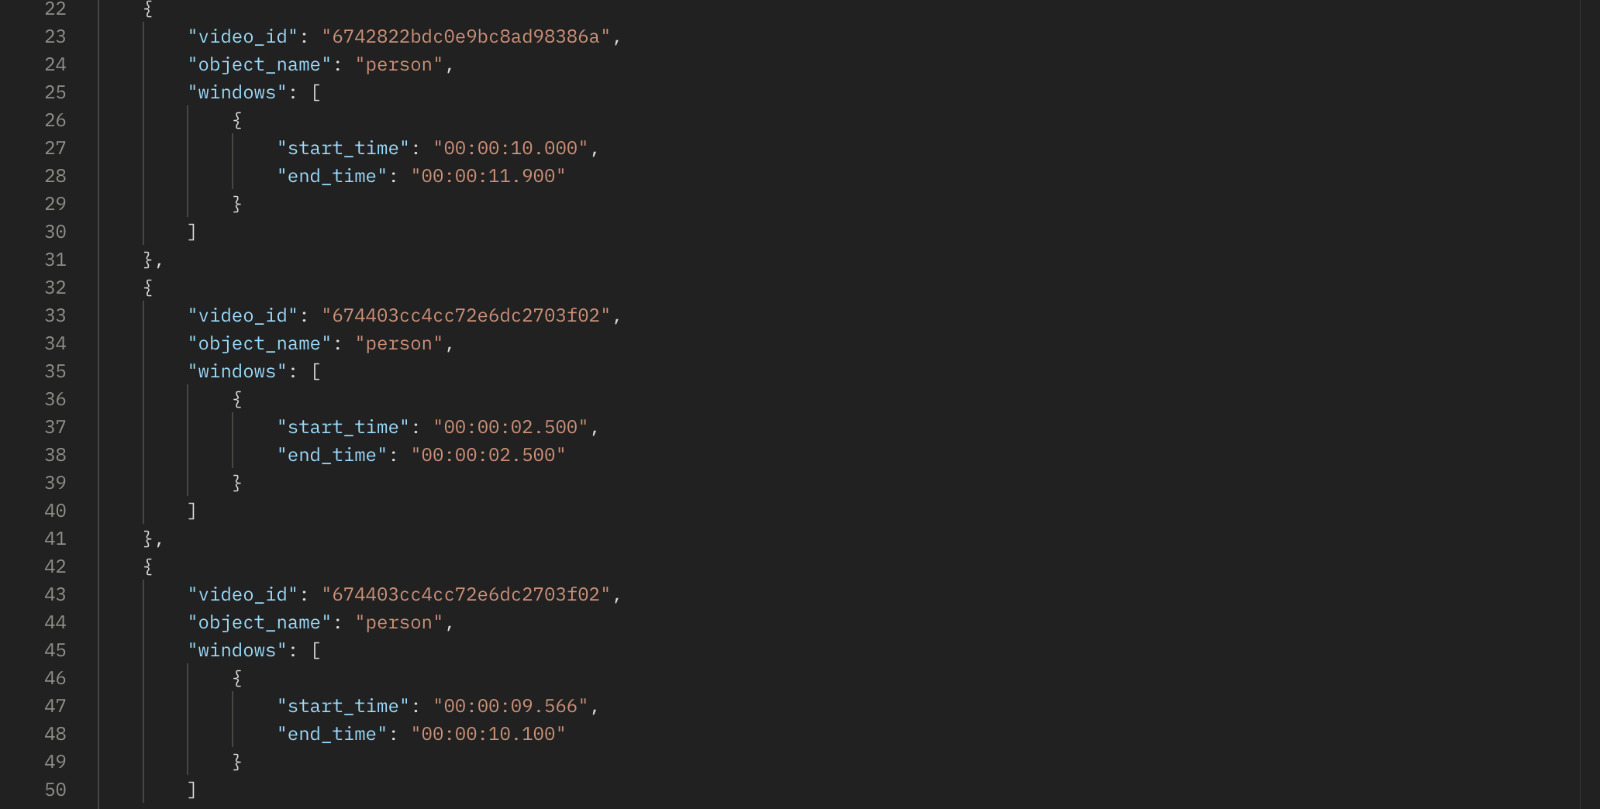
\includegraphics[width=0.45\textwidth]{2.jpeg}
    \caption{Result of spatial query for person in bottom right}
    \label{fig:query2}
\end{figure}

\subsection{Spatial Objects AND Query}
\textbf{Endpoint:} \\ 
\texttt{/query/spatialObjectsAnd}

This endpoint implements logical AND operations to find video segments where multiple objects appear simultaneously in the specified area.

\textbf{Parameters:}
\begin{itemize}
    \item \texttt{objects}: Array of object names (minimum 2 objects required)
    \item \texttt{area}: Predefined area or custom box coordinates
\end{itemize}

Example queries:\\
\begin{minipage}{\linewidth}
\scriptsize
\begin{verbatim}
/query/spatialObjectsAnd?objects=["person","truck","dog"]
&area=left-half
\end{verbatim}
\end{minipage}

\begin{figure}[H]
    \centering
    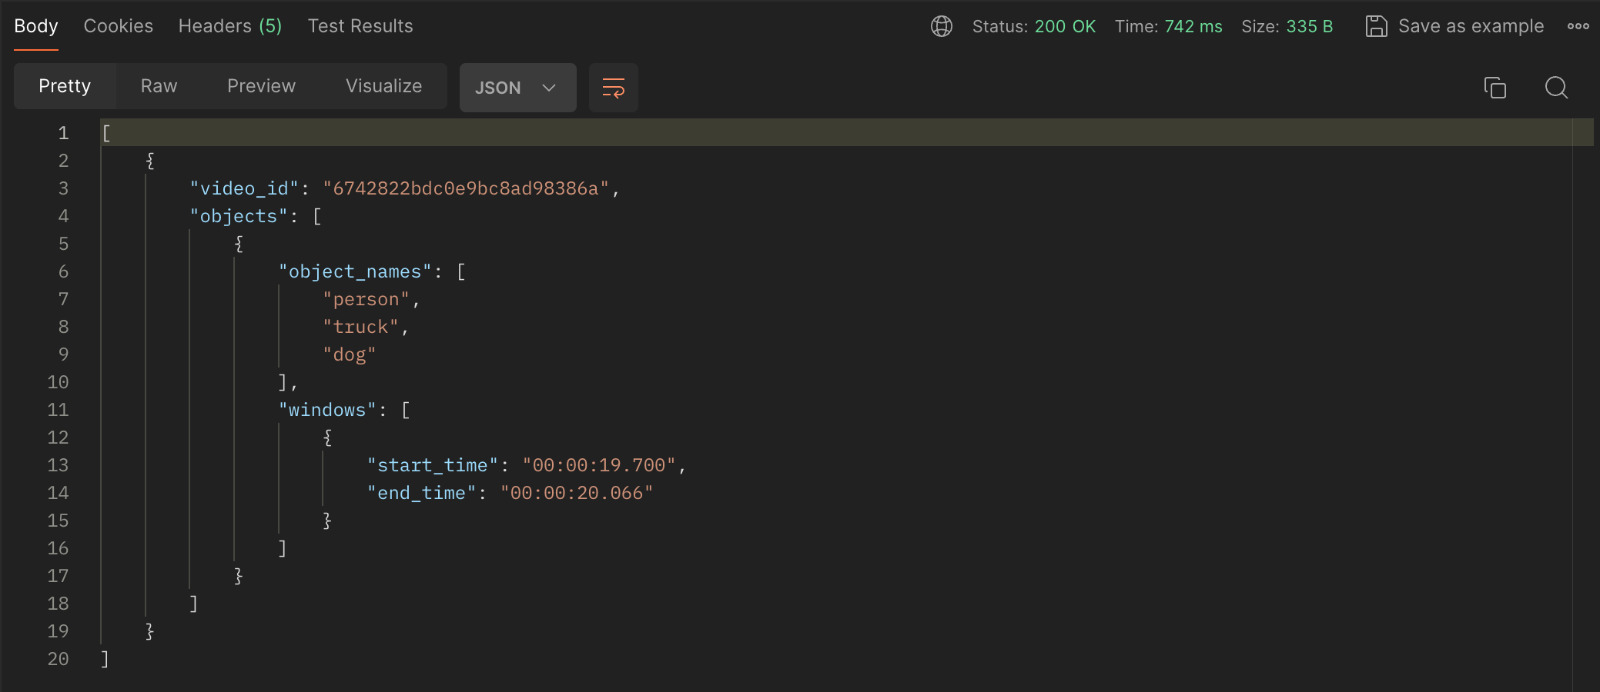
\includegraphics[width=0.45\textwidth]{3.jpeg}
    \caption{Result of AND query for person, truck, and dog in left half}
    \label{fig:query3}
\end{figure}

\begin{minipage}{\linewidth}
\scriptsize
\begin{verbatim}
/query/spatialObjectsAnd?objects=["person","truck"]
&area=left-half
\end{verbatim}
\end{minipage}

\begin{figure}[H]
    \centering
    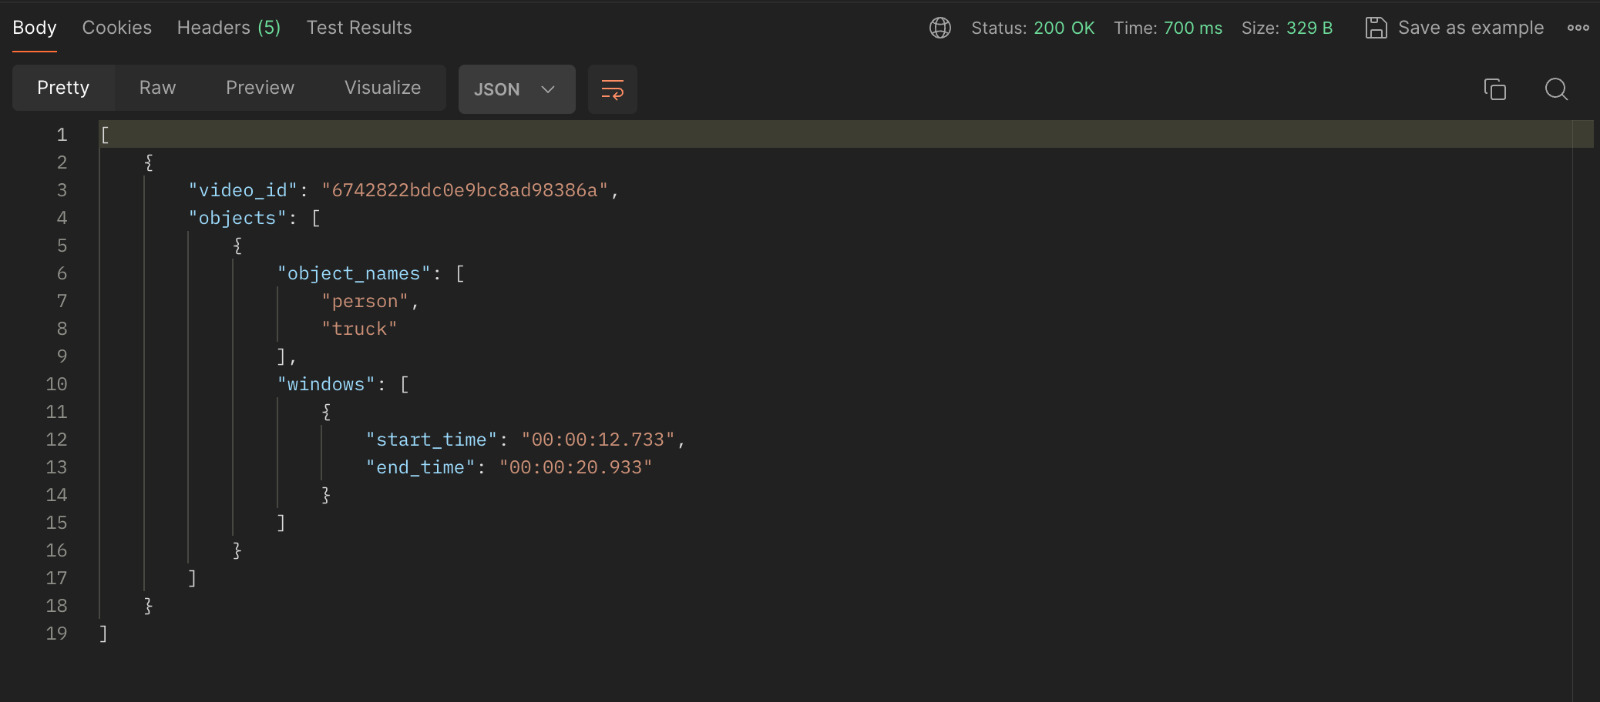
\includegraphics[width=0.45\textwidth]{4.jpeg}
    \caption{Result of AND query for person and truck in left half}
    \label{fig:query4}
\end{figure}

\subsection{Instance-Based Queries}
\subsubsection{Distinct Instances Query}
\textbf{Endpoint:} \\ 
\texttt{/query/queryDistinctInstances}

Retrieves all individual instances of a specified object class across all videos.

Example query:\\
\begin{minipage}{\linewidth}
\scriptsize
\begin{verbatim}
/query/queryDistinctInstances?object=person
\end{verbatim}
\end{minipage}

\begin{figure}[H]
    \centering
    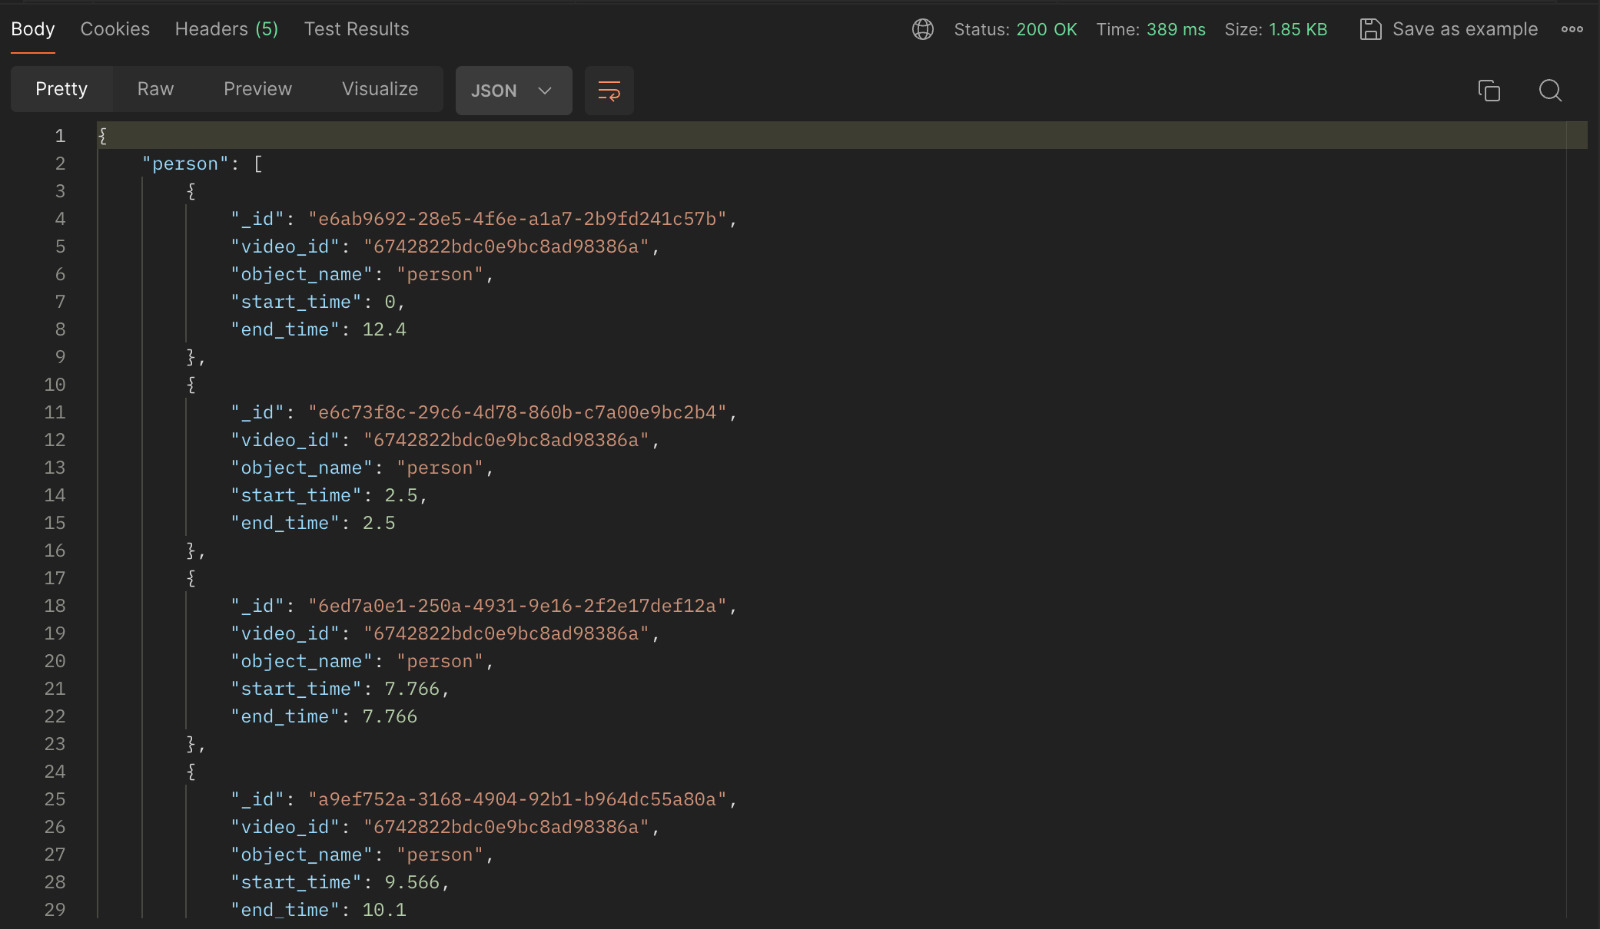
\includegraphics[width=0.45\textwidth]{5.jpeg}
    \caption{Result of distinct instances query for person}
    \label{fig:query5}
\end{figure}

\subsubsection{Instance Overlaps Query}
\textbf{Endpoint:} \\ 
\texttt{/query/queryInstanceOverlaps}

Identifies temporal windows where multiple instances of the same object class appear simultaneously.

\textbf{Parameters:}
\begin{itemize}
    \item \texttt{object}: Object class name
    \item \texttt{count}: Minimum number of simultaneous instances
\end{itemize}

Example queries:\\
\begin{minipage}{\linewidth}
\scriptsize
\begin{verbatim}
/query/queryInstanceOverlaps?object=person&count=3
\end{verbatim}
\end{minipage}

\begin{figure}[H]
    \centering
    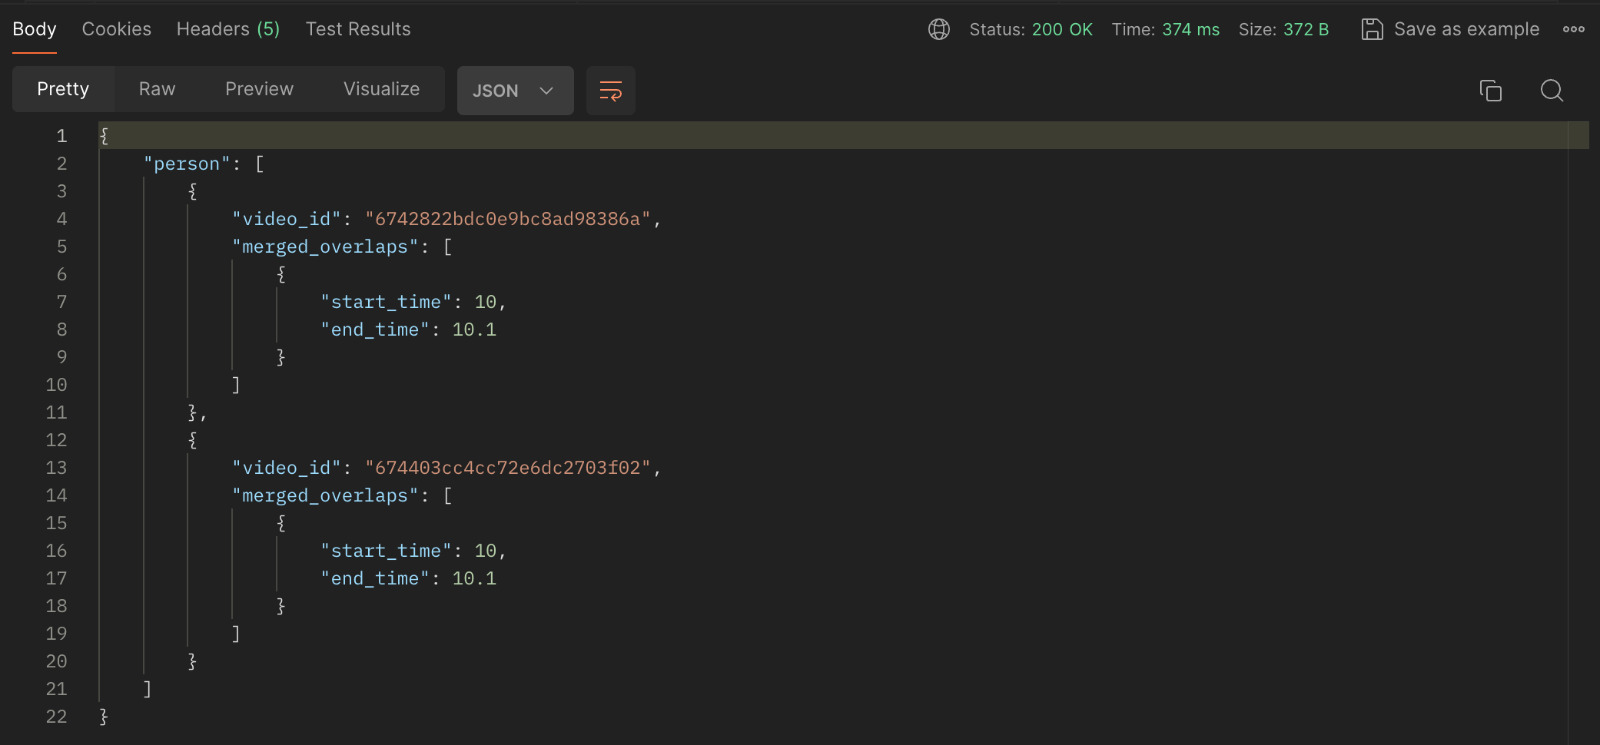
\includegraphics[width=0.45\textwidth]{6.jpeg}
    \caption{Result of instance overlaps query for 3 persons}
    \label{fig:query6}
\end{figure}

\begin{minipage}{\linewidth}
\scriptsize
\begin{verbatim}
/query/queryInstanceOverlaps?object=person&count=2
\end{verbatim}
\end{minipage}

\begin{figure}[H]
    \centering
    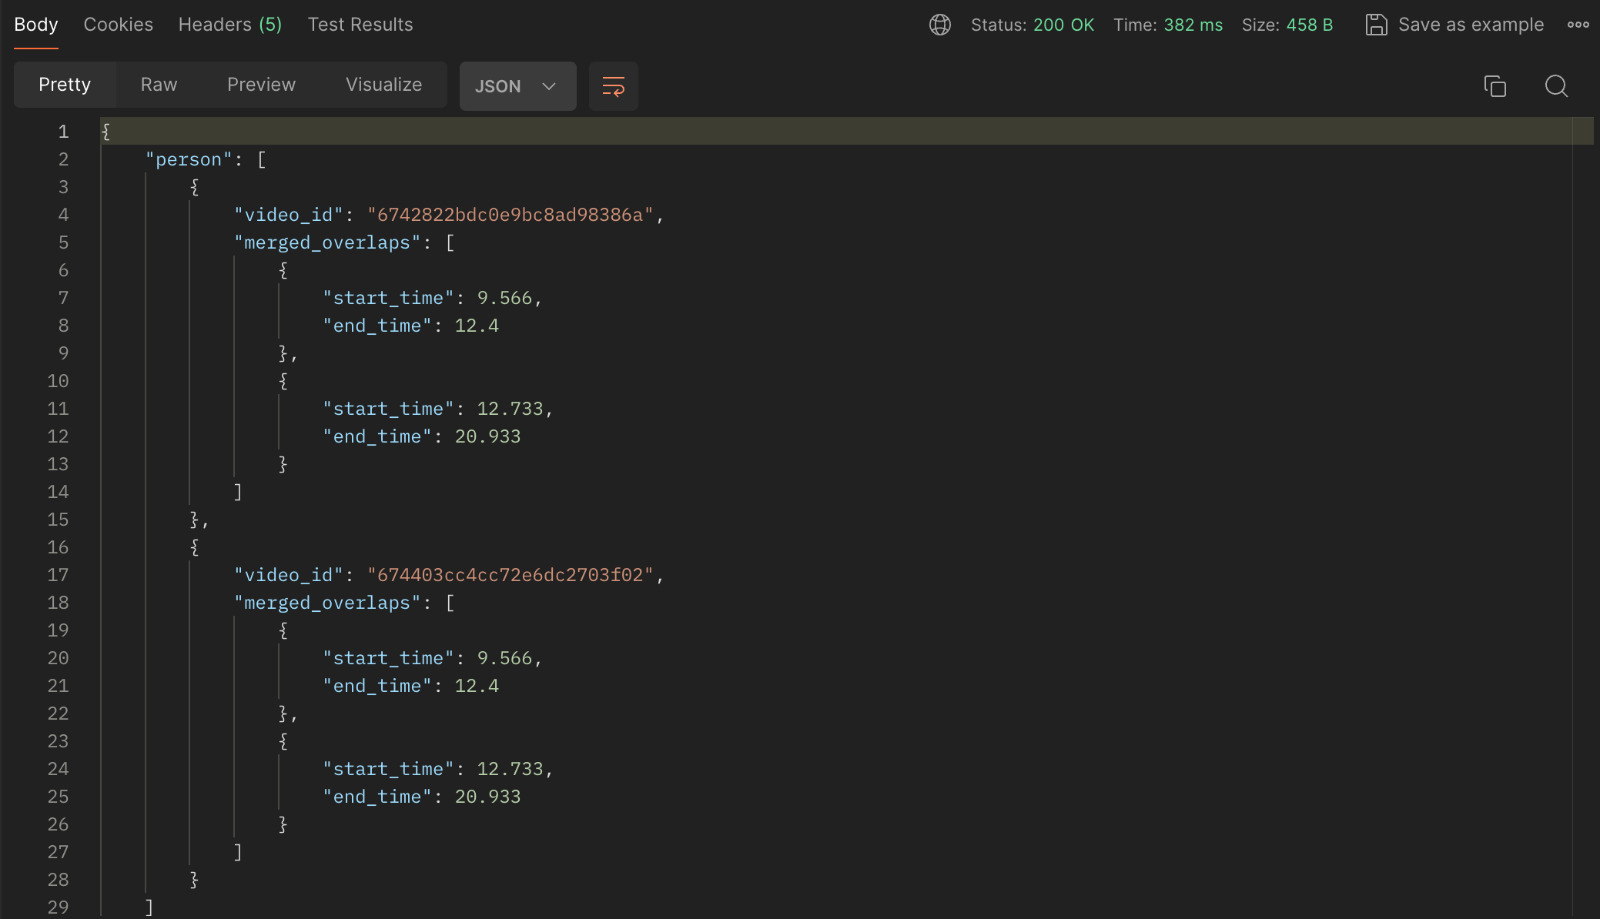
\includegraphics[width=0.45\textwidth]{7.jpeg}
    \caption{Result of instance overlaps query for 2 persons}
    \label{fig:query7}
\end{figure}

\subsubsection{Instance Overlaps in Area Query}
\textbf{Endpoint:} \\ 
\texttt{/query/queryInstanceOverlapsInArea}

Extends the instance overlaps query by adding spatial constraints, finding multiple instances of the same object class within a specified area.

Example queries:\\
\begin{minipage}{\linewidth}
\scriptsize
\begin{verbatim}
/query/queryInstanceOverlapsInArea?object=person
&count=2&area=top-right
\end{verbatim}
\end{minipage}

\begin{figure}[H]
    \centering
    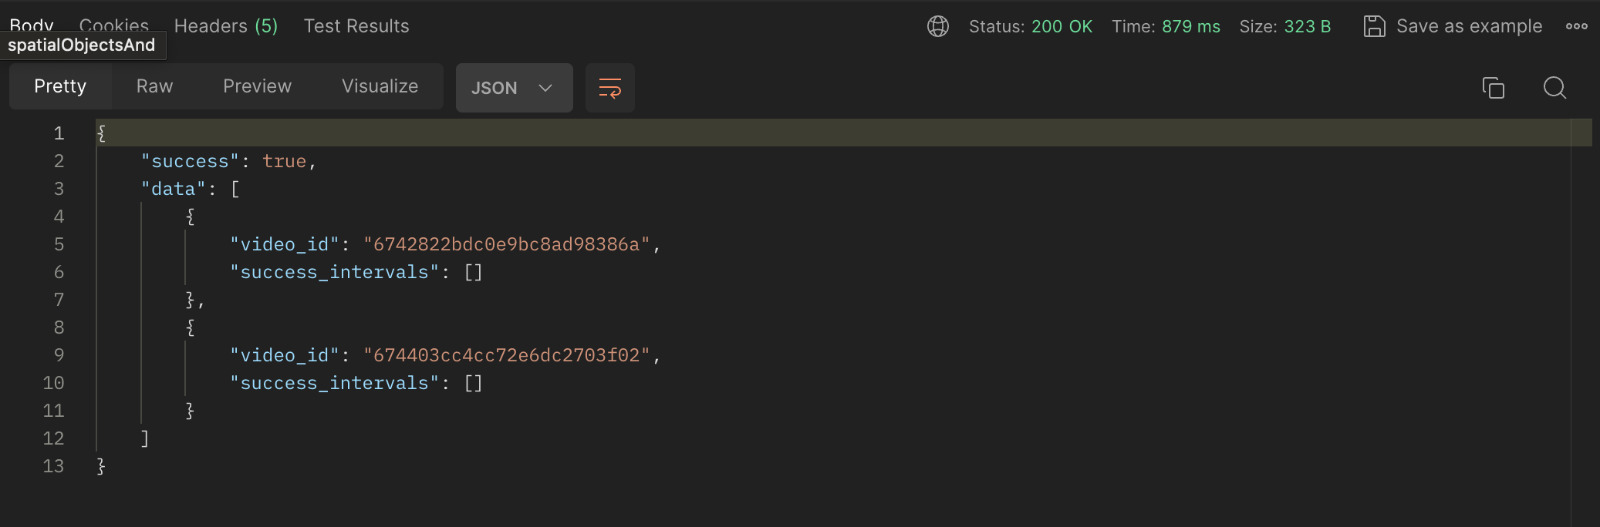
\includegraphics[width=0.45\textwidth]{8.jpeg}
    \caption{Result of instance overlaps in top-right area}
    \label{fig:query8}
\end{figure}

\begin{minipage}{\linewidth}
\scriptsize
\begin{verbatim}
/query/queryInstanceOverlapsInArea?object=person
&count=2&area=left-half
\end{verbatim}
\end{minipage}

\begin{figure}[H]
    \centering
    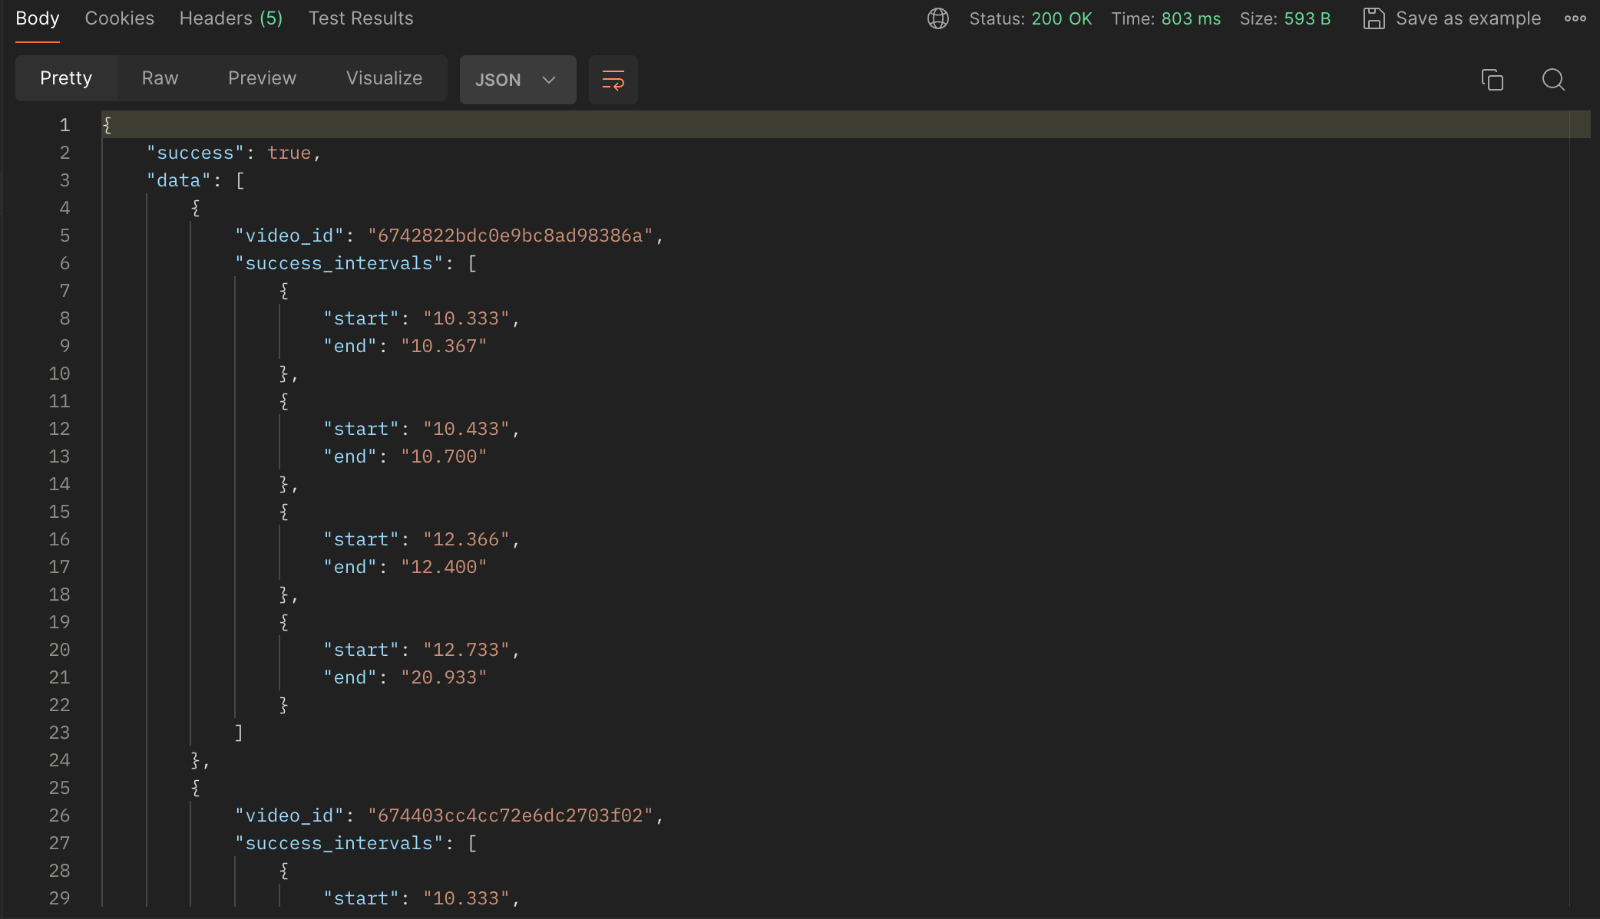
\includegraphics[width=0.45\textwidth]{9.jpeg}
    \caption{Result of instance overlaps in left-half area}
    \label{fig:query9}
\end{figure}

\subsection{Temporal Queries}
\textbf{Endpoint:} \\ 
\texttt{/query/queryInstancesAtTime}

Retrieves all instances of specified objects at a particular timestamp.

\textbf{Parameters:}
\begin{itemize}
    \item \texttt{object}: Object class name
    \item \texttt{time}: Timestamp in seconds
\end{itemize}

Example queries:\\
\begin{minipage}{\linewidth}
\scriptsize
\begin{verbatim}
/query/queryInstancesAtTime?object=person&time=2
\end{verbatim}
\end{minipage}

\begin{figure}[H]
    \centering
    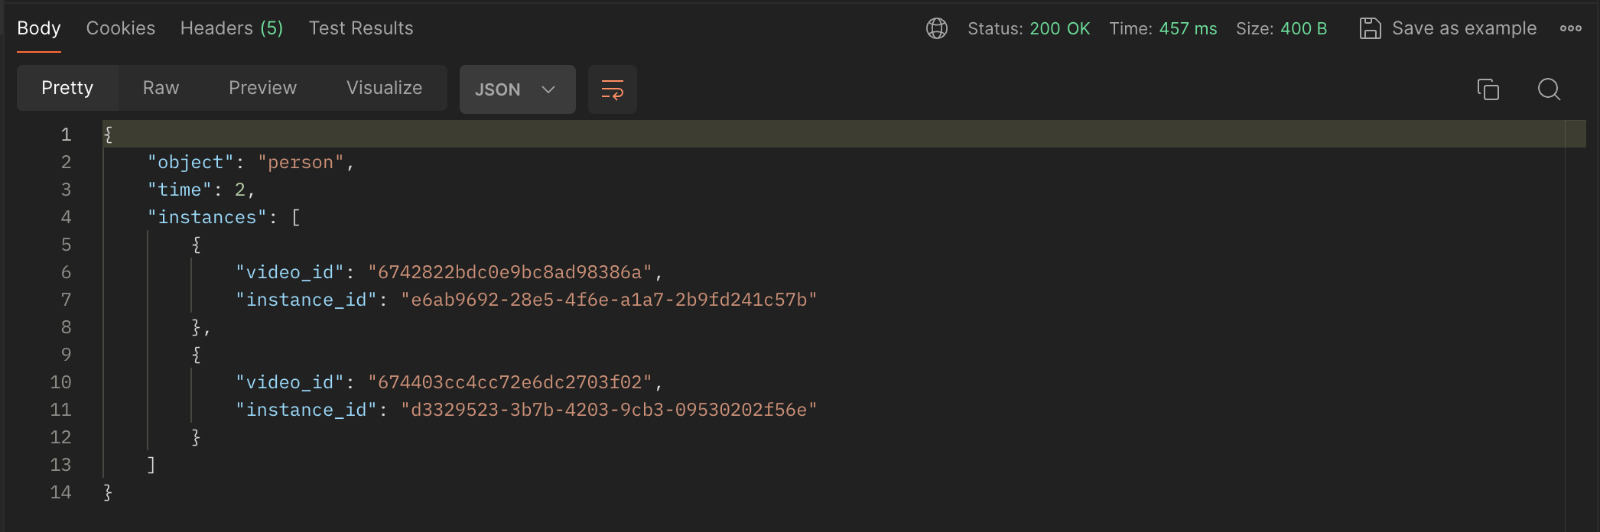
\includegraphics[width=0.45\textwidth]{10.jpeg}
    \caption{Result of temporal query at 2 seconds}
    \label{fig:query10}
\end{figure}

\begin{minipage}{\linewidth}
\scriptsize
\begin{verbatim}
/query/queryInstancesAtTime?object=person&time=13
\end{verbatim}
\end{minipage}

\begin{figure}[H]
    \centering
    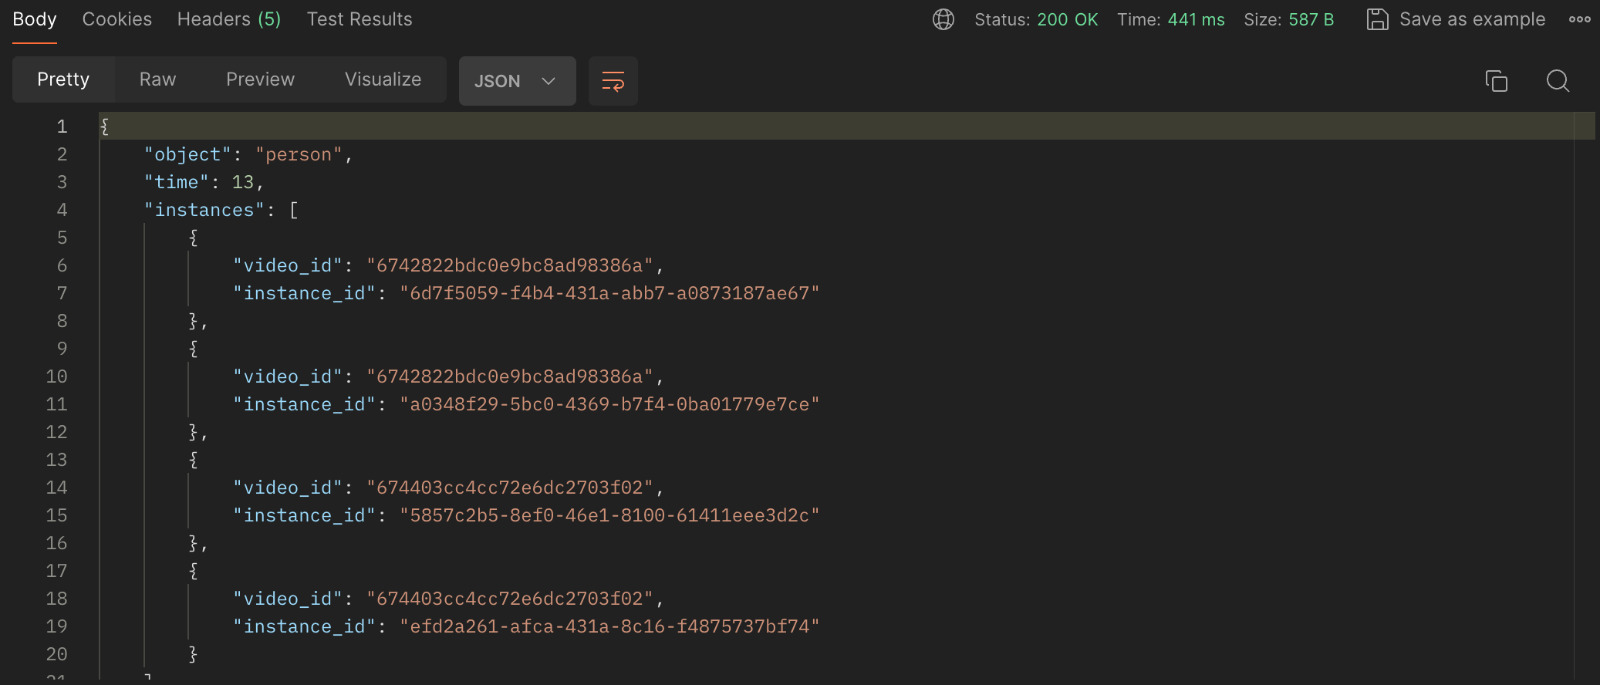
\includegraphics[width=0.45\textwidth]{11.jpeg}
    \caption{Result of temporal query at 13 seconds}
    \label{fig:query11}
\end{figure}
\begin{table}[h!]
    \centering
    \begin{tabular}{|l|l|}
        \hline
        \textbf{Query Name} & \textbf{Query Time} \\ \hline
        spatialObjects & 438 ms \\ \hline
        spatialObjectsAnd & 700 ms \\ \hline
        queryDistinctInstances & 389 ms \\ \hline
        queryInstanceOverlaps & 382 ms \\ \hline
        queryInstanceOverlapsInArea & 803 ms \\ \hline
        queryInstancesAtTime & 441 ms \\ \hline
        object & 1101 ms \\ \hline
        spatialObjectsTemporal & 416 ms \\ \hline
    \end{tabular}
    \caption{Query performance average times for various query types}
    \label{tab:query_times}
\end{table}
\begin{table}[h!]
    \centering
    \begin{tabular}{|l|l|l|}
        \hline
        \textbf{Systems} & \textbf{Prediction Accuracy} \\ \hline
        Google Cloud Video Intelligence API & 80-90\% \\ \hline
        Yolo 11 & 79\% \\ \hline
    \end{tabular}
    \caption{Prediction Accuracy Comparison with Systems.}
    \label{tab:prediction_accuracy}
\end{table}
These query endpoints demonstrate the system's capability to perform complex spatial-temporal searches across video content, enabling precise retrieval of relevant video segments based on object presence, location, and timing requirements.


\section{Challenges and Limitations}
\label{sec:challenges}

\subsection{Challenges}
\label{sec:challenges-sub}

This project faced several challenges, particularly in transitioning from TransVOD++ to YOLOv11. TransVOD++, while optimized for spatiotemporal video analysis, exhibited significant limitations in object detection across diverse scenarios. For instance:
\begin{itemize}
    \item \textbf{Narrow Object Detection Scope:} TransVOD++ reliably detected specific objects (e.g., a "husk") but struggled with generic object classes such as an "apple," limiting its utility in broader applications.
    \item \textbf{Complexity of Integration:} Its focus on temporal and spatial modeling made it challenging to align with our metadata generation pipeline, which prioritizes explicit object recognition.
\end{itemize}

In contrast, YOLOv11 was chosen for its robust neural architecture search (NAS) capabilities and transformer-based enhancements, which significantly improved detection accuracy and query responsiveness. However, integrating YOLOv11 into a scalable framework required careful adjustments to the pipeline, including adapting it to handle varying video resolutions and object densities.

Additionally, handling metadata storage and retrieval in MongoDB GridFS posed logistical hurdles. Optimizing the chunk size to 5 MB minimized overhead, but this approach still poses challenges with larger video files, as chunk size may need further re-evaluation to maintain efficiency.


\subsection{Limitations}
\label{sec:limitations}

The current approach, while demonstrating significant advancements, has notable limitations:

\begin{itemize}
    \item \textbf{Limited Object Detection Scope:} The reliance on a pre-trained YOLO11 model constrains the system to detecting a predefined set of objects from the COCO dataset. This limitation restricts applicability in domains requiring the identification of custom or specialized object types.
    \item \textbf{Pipeline Integration Challenges:} Existing video processing pipelines like Scanner \cite{poms2018scanner}, which could enhance video processing efficiency, are no longer actively developed. Attempts to integrate these tools revealed compatibility issues with our workflow.
    \item \textbf{GridFS Chunk Size Management:} While the default 255 KB chunk size in GridFS was optimized to 5 MB to reduce metadata overhead, this solution may not scale well for significantly larger video files. Dynamic evaluation of chunk sizes is necessary to balance storage and retrieval efficiency.
    \item \textbf{Absence of Advanced Features:} The system does not yet handle cross-model collaboration or provide real-time updates. Implementing these features would require substantial architectural enhancements.
\end{itemize}

Despite these limitations, the system lays a solid foundation for future enhancements. Addressing these areas will unlock its potential for diverse applications, including autonomous systems, large-scale surveillance, and AI-driven content recommendation.

\label{sec:limitations-sub}








\section{Conclusions and Future Work}
\label{sec:conclusions}
\subsection{Conclusions}
In this project, we presented a novel video querying system designed to address the challenges of processing and analyzing large-scale video datasets. Our approach integrates advanced object detection and metadata generation techniques to enable precise spatial-temporal queries and multi-object interaction detection.
Key achievements of the system include:
\begin{itemize}
    \item Leveraging MongoDB for metadata storage, enabling efficient querying and retrieval.
    \item Utilizing FFmpeg for keyframe-based video fragmentation to optimize storage and scalability.
    \item Enhancing the querying process to support diverse use cases, such as autonomous driving and surveillance.
\end{itemize}

While the system demonstrates significant advancements in video analysis and querying, certain limitations remain. These include reliance on a pre-trained YOLO11 model constrained by its training dataset, the absence of parallel processing for multiple machine learning models, and challenges in leveraging pipelines such as Scanner. Addressing these constraints offers exciting directions for future development.

The proposed framework lays the foundation for scalable and efficient video analysis systems, with potential applications in autonomous driving, surveillance, and content recommendation. Future enhancements, such as incorporating dynamic chunking strategies, spatial indexing, and cross-model collaboration, can further elevate the system's capabilities, making it a valuable tool for researchers and engineers working with large-scale video datasets.

\label{sec:future-work-sub}
\subsection{Future Work}
To further enhance the system, future work will focus on:
\begin{itemize}
    \item \textbf{Advanced Scene-Text Grounding:} Integrating neural architectures and contextual embeddings for precise text extraction from video frames, enabling applications like automated indexing, real-time text recognition, and semantic video search.
    \item \textbf{Parallel Model Integration:} Enabling the concurrent execution of multiple machine learning models by introducing additional status states within the video processing pipeline, thereby generating richer metadata.
    \item \textbf{Spatial and Temporal Indexing:} Employing advanced indexing techniques to accelerate spatial-temporal queries, particularly in large datasets requiring complex object interaction analysis.
\end{itemize}

These improvements will significantly enhance the system's utility, making it a more versatile and impactful tool for researchers and engineers working with large-scale video datasets.


\section{Technical Details and Algorithms}
\subsection{Object Tracking}
\subsubsection{Overview of Object Tracking}
The provided implementation performs object tracking in videos using the YOLO (You Only Look Once) object detection model. The key objectives are:
\begin{itemize}
    \item Detect objects in each video frame.
    \item Maintain a consistent identity for each detected object across frames.
    \item Handle multiple instances of the same object type.
\end{itemize}

\subsubsection{Key Components of Object Tracking}

\subsubsection{Object Detection}
The YOLO model detects objects in each frame and provides the following:
\begin{itemize}
    \item Bounding boxes $B$ represent the location of detected objects in the frame.
    \item Class labels $L$ indicating the type of object (e.g., person, car).
    \item Confidence scores $C$ for each detection.
\end{itemize}

\subsubsection{Active Object Tracking}
Detected objects are stored in an \texttt{active\_objects} dictionary, which tracks each object’s state, including:
\begin{itemize}
    \item A unique identifier $\text{instance\_id}$.
    \item The last frame and timestamp the object was seen.
    \item The bounding box $B$ of the object.
\end{itemize}

\subsubsection{Intersection over Union (IoU)}
To associate detections across frames, the Intersection over Union (IoU) metric is used. IoU measures the overlap between two bounding boxes $B_1$ and $B_2$. Mathematically, it is defined as:
\begin{equation}
\text{IoU} = \frac{|B_1 \cap B_2|}{|B_1 \cup B_2|},
\end{equation}
where $|B_1 \cap B_2|$ is the area of intersection and $|B_1 \cup B_2|$ is the area of the union of the two bounding boxes. An IoU threshold $\tau$ is used to determine if two bounding boxes represent the same object.

\subsubsection{Timeout and Object Expiry}
To handle objects disappearing from the frame temporarily, a timeout threshold $T_{\text{timeout}}$ is used. If an object is not detected for a duration exceeding $T_{\text{timeout}}$, it is removed from the \texttt{active\_objects} dictionary.

\subsubsection{Handling Multiple Instances of the Same Object Type}
When multiple objects of the same class are present, the implementation distinguishes them using the following steps:

\subsubsection{Label-Based Grouping}
Detected objects are grouped by their class label $L$. Each class label maintains its own list of active objects.

\subsubsection{IoU-Based Association}
For each detected object in the current frame, the IoU is computed with all active objects of the same label. Let $B_t$ be the bounding box of a detected object at time $t$, and $B_{t-1}$ be the bounding box of a previously tracked object. If:
\begin{equation}
\text{IoU}(B_t, B_{t-1}) > \tau,
\end{equation}
then $B_t$ is associated with the same object as $B_{t-1}$.

\subsubsection{New Object Creation}
If no existing object satisfies the IoU threshold, a new object is created with a unique identifier $\text{instance\_id}$ and added to \texttt{active\_objects}.

\subsubsection{Relative Position Calculation}
The relative position of an object in the frame is calculated as:
\begin{equation}
\text{Relative Position} = \left( \frac{x_{\text{center}}}{W}, \frac{y_{\text{center}}}{H} \right),
\end{equation}
where $x_{\text{center}} = \frac{x_1 + x_2}{2}$ and $y_{\text{center}} = \frac{y_1 + y_2}{2}$. Here, $x_1, y_1, x_2, y_2$ are the coordinates of the bounding box, and $W, H$ are the frame width and height, respectively.

\subsubsection{Data Storage and Updates}
Each object’s data is stored in a MongoDB collection, including:
\begin{itemize}
    \item Bounding box coordinates $B$.
    \item Confidence score $C$.
    \item Relative position.
    \item Start and end timestamps.
\end{itemize}

When an object is matched in a new frame, its entry in the database is updated with the latest data.

\subsubsection{Conclusion}
This implementation effectively tracks objects across video frames using a combination of:
\begin{itemize}
    \item Detection via YOLO.
    \item IoU-based matching for consistent identification.
    \item Timeout thresholds for handling occlusions.
    \item MongoDB for persistent storage.
\end{itemize}
These methods enable reliable tracking of multiple instances of the same class and ensure accurate object identification throughout the video.



% FRAGMENTATION

\subsection{Efficient Video Fragmentation and Retrieval}

The proposed system incorporates a novel approach for video fragmentation, leveraging keyframes to divide videos into smaller, approximately 5-second chunks. This method is essential for optimizing the storage and retrieval of video data, particularly for large-scale datasets. 

\subsubsection{Keyframe-Based Fragmentation}
Keyframes, or intra-frames, are self-contained frames that do not rely on other frames for decoding. The fragmentation process ensures that video chunks are split at keyframes, avoiding visual artifacts and ensuring compatibility with playback tools. The system uses FFmpeg to achieve this, with the following characteristics:
\begin{itemize}
    \item \textbf{No Transcoding/Re-Encoding}: By copying the codec (\texttt{-codec copy}), the video quality remains intact, and computational overhead is minimized.
    \item \textbf{Variable Chunk Lengths}: Chunks align with the nearest keyframe after the specified duration (e.g., 5 seconds), ensuring the integrity of each segment.
\end{itemize}

\subsubsection{Metadata for Precise Retrieval}
Each video chunk is associated with metadata stored in MongoDB GridFS, including:
\begin{itemize}
    \item \textbf{Video ID}: Identifies the original video.
    \item \textbf{Start and End Timestamps}: Denote the temporal boundaries of the chunk.
    \item \textbf{Duration}: Specifies the length of the fragment.
\end{itemize}
This metadata facilitates temporal and spatial queries, enabling efficient access to specific segments without processing the entire video.

\subsubsection{Advantages of Fragmentation}
The fragmentation approach offers several benefits:
\begin{itemize}
    \item \textbf{Efficient Bandwidth Usage}: Only relevant chunks are transmitted, significantly reducing network load compared to retrieving whole video files.
    \item \textbf{Scalable Storage}: Parallel processing of chunks improves system scalability for large datasets.
    \item \textbf{Optimized Querying}: Metadata enables rapid temporal and spatial searches, essential for applications requiring precise video segment retrieval.
    \item \textbf{Improved User Experience}: Users can access desired segments quickly, enhancing interactivity and responsiveness.
\end{itemize}


% END OF ALGORITHMS

\bibliographystyle{IEEEtran}
\bibliography{references}

\end{document}
